\chapter{Projekt i implementacja aplikacji}

\section{Funkcje aplikacji - diagram przypadków użycia}

\begin{figure} [H]
	\centering
	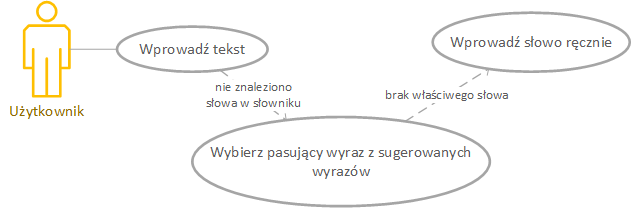
\includegraphics[width=1\linewidth]{rozdzial03/diagram.png}
	\caption{Diagram przypadków użycia}
	\label{fig:diagUzycia}
\end{figure}

Głównym zadaniem aplikacji jest wyszukiwanie błędnych wyrazów w języku polskim oraz ich korekcja. Aby tego dokonać aplikacja porównuje wyrazy znajdujące się w tekście z wyrazami znajdującymi się w słowniku. Jeśli danego słowa nie znaleziono zostaje ono uznane za błędne. Aby dokonać korekcji błędnych wyrazów stosowane są algorytmy opisane w poprzednich rozdziałach. Dla optymalizacji działania aplikacji wyszukiwanie sugestii odbywa się w osobnych wątkach co znacząco przyspiesza działanie aplikacji. 


\section{Interfejs aplikacji}

\begin{figure} [H]
	\centering
	\includegraphics[width=1\linewidth]{rozdzial03/screen1_1.png}
	\caption{Interfejs aplikacji}
	\label{fig:interfejs}
\end{figure}

\begin{enumerate}
	\item Ilość podpowiedzi - pozwala na ustawienie maksymalnej ilości podpowiedzi jakie mają się pojawić po kliknięciu prawym przyciskiem myszy na błędnie napisane słowo.
	\item Odległość Levenhteina - pozwala na ustawienie odległości jaka ma być brana pod uwagę w przypadku algorytmu Levenhstaina. Im większa liczba tym więcej podpowiedzi ale jednocześnie zmniejsza to szybkość działania aplikacji ze względu na dodatkowe obliczenia które muszą zostać wykonane. 
	\item Ilość zmian - pozwala na ustawienie parametru ilości zmian dla algorytmu podmieniającego znaki diakrytyczne. Im większa liczba tym więcej podpowiedzi oraz dłuższy czas wykonywania algorytmu.
	\item Edytor tekstu - pozwala na edycję tekstu. Wyszukiwanie błędów działa w czasie rzeczywistym (funkcja sprawdzająca poprawność uruchamia się z każdym kliknięciem spacji). Jeśli dane słowo zostało uznane za błędne zostaje zaznaczone kolorem czerwonym. Aby je poprawić należy kliknąć na nie prawym przyciskiem myszki. Zostanie wyświetlone menu kontekstowe zawierające możliwe zamienniki. Aby podmienić słowo wystarczy kliknąć na zamiennik. Możliwe jest również poprawienie tekstu ręcznie wpisując w miejscu błędnego słowa poprawne. 
	
\end{enumerate}

\section{Wpływ parametrów na wyniki wyszukiwania}

\begin{figure} [H]
	\centering
	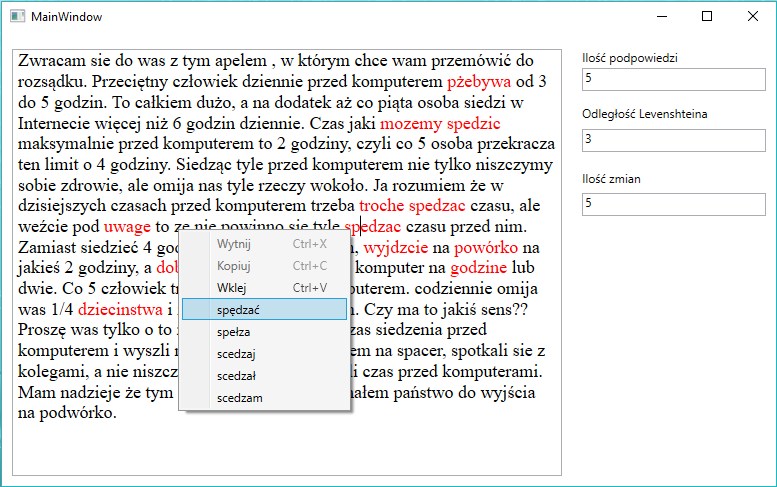
\includegraphics[width=1\linewidth]{rozdzial03/screen2.png}
	\caption{Przykładowy wynik wyszukiwania sugestii}
	\label{fig:interfejs1}
\end{figure}

\begin{figure} [H]
	\centering
	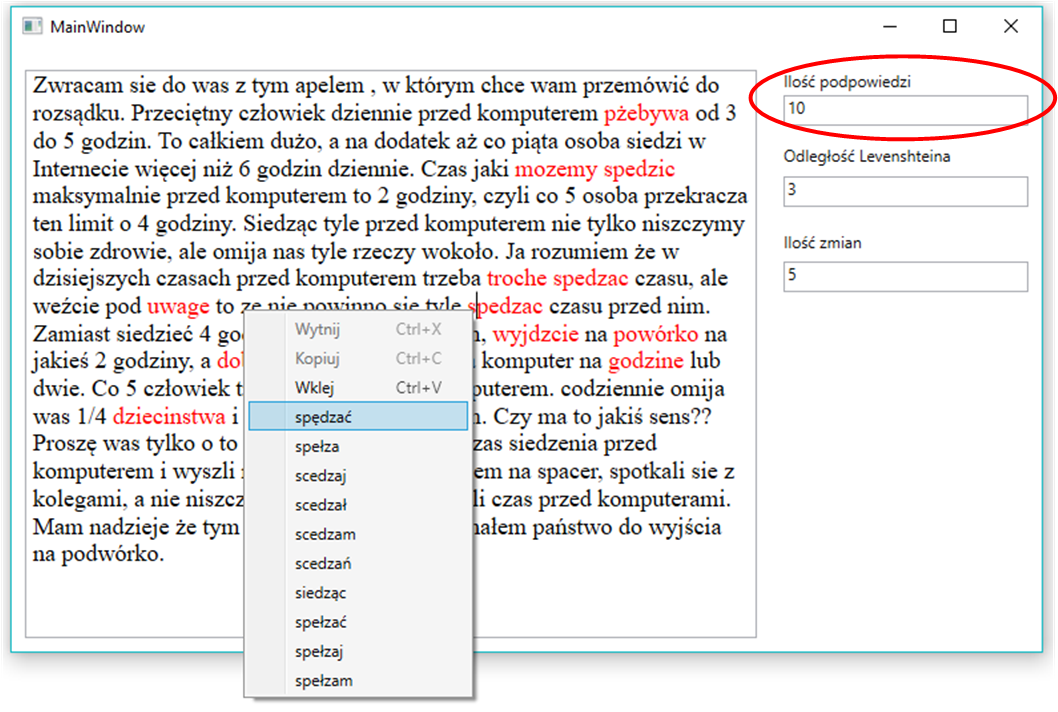
\includegraphics[width=1\linewidth]{rozdzial03/screen3_1.png}
	\caption{Zwiększenie ilości wyświetlanych sugestii}
	\label{fig:interfejs2}
\end{figure}

\begin{figure} [H]
	\centering
	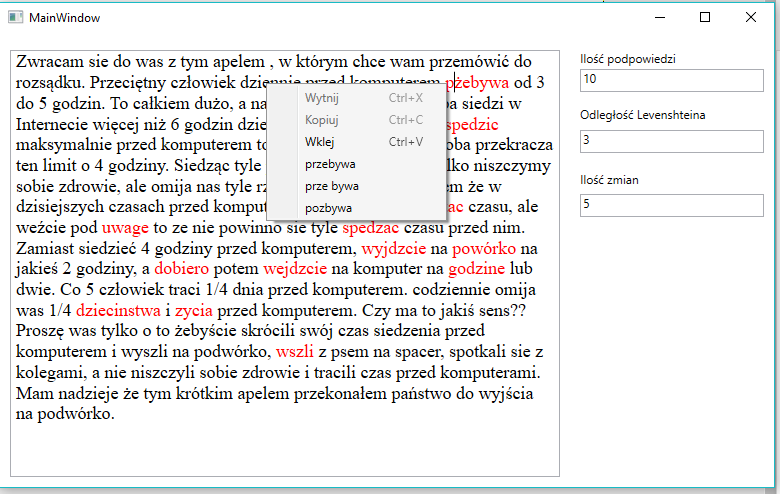
\includegraphics[width=1\linewidth]{rozdzial03/screen4.png}
	\caption{Przykładowy wynik wyszukiwania sugestii dla małej ilości podpowiedzi}
	\label{fig:interfejs3}
\end{figure}

\begin{figure} [H]
	\centering
	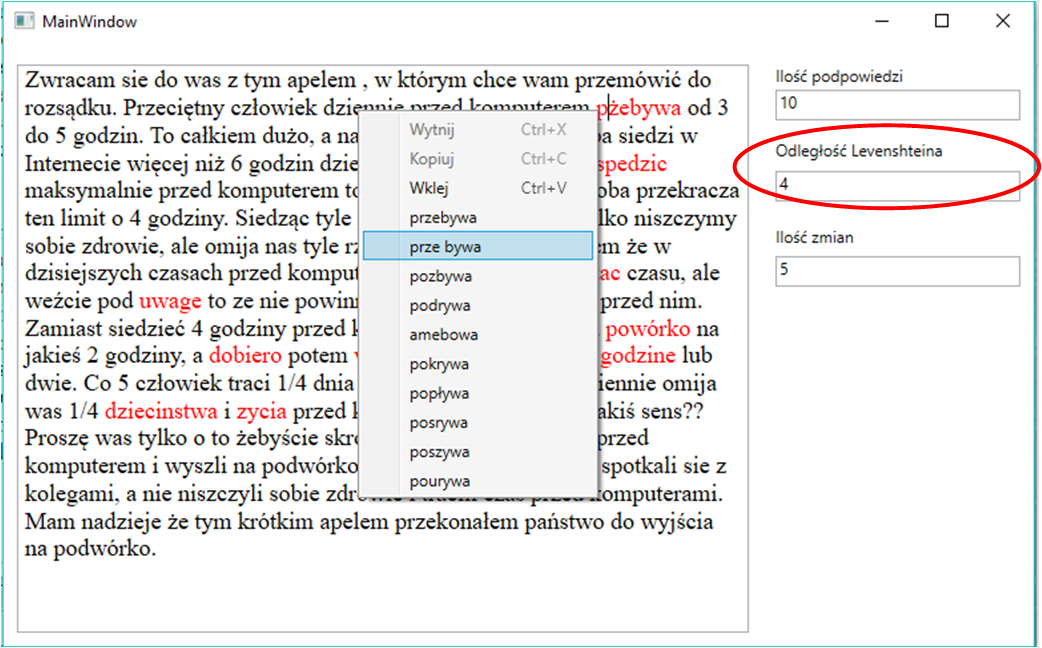
\includegraphics[width=1\linewidth]{rozdzial03/screen5_1.png}
	\caption{Zwiększenie odległości Levenhstaina}
	\label{fig:interfejs4}
\end{figure}

\begin{figure} [H]
	\centering
	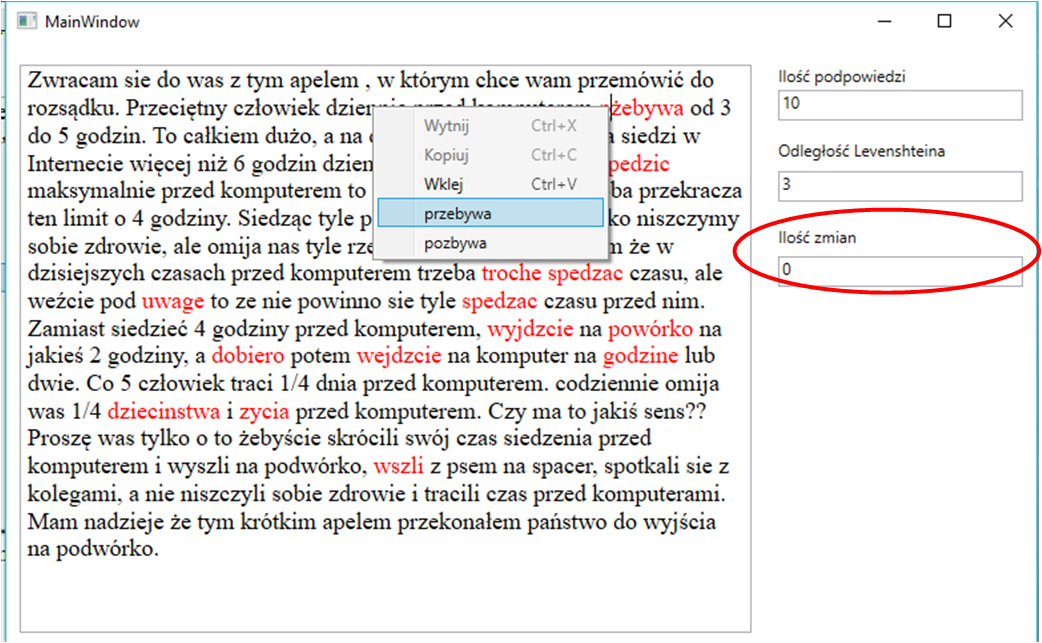
\includegraphics[width=1\linewidth]{rozdzial03/screen6_1.png}
	\caption{Zwiększenie ilości zmian}
	\label{fig:interfejs5}
\end{figure}

Odpowiednio zmieniając parametry znajdujące się w prawej części okna aplikacji można dostosować wyszukiwanie do potrzeb użytkownika. Rysunek \ref{fig:interfejs1} przedstawia przykładowe wyniki wyszukiwania podpowiedzi. Jeśli ilość wyświetlanych wyników nie jest odpowiednia można zmienić ich ilość tak aby uzyskać satysfakcjonujący wynik. Rysunek \ref{fig:interfejs2} przedstawia wpływ zwiększenia ilości wyświetlanych podpowiedzi. Jednocześnie ilość podpowiedzi nie ma wpływu na szybkość działania aplikacji. 

Pozostałe parametry wpływają na podobieństwo sugestii do wprowadzonego błędnie słowa. Na rysunku \ref{fig:interfejs3} został przedstawiony przykładowy wynik wyszukiwania który przy danych parametrach nie wypełnia całej listy podpowiedzi. Na rysunku \ref{fig:interfejs4} zwiększono odległość Levenhstaina tak aby uzyskać więcej sugestii. Natomiast na rysunku \ref{fig:interfejs5} całkowicie zminimalizowano wpływ algorytmu podmieniającego znaki tak aby pozbyć się niechcianych podpowiedzi zawierających spacje.
 
\section{Realizacja wybranych funkcjonalności}

\begin{figure} [H]
	\centering
	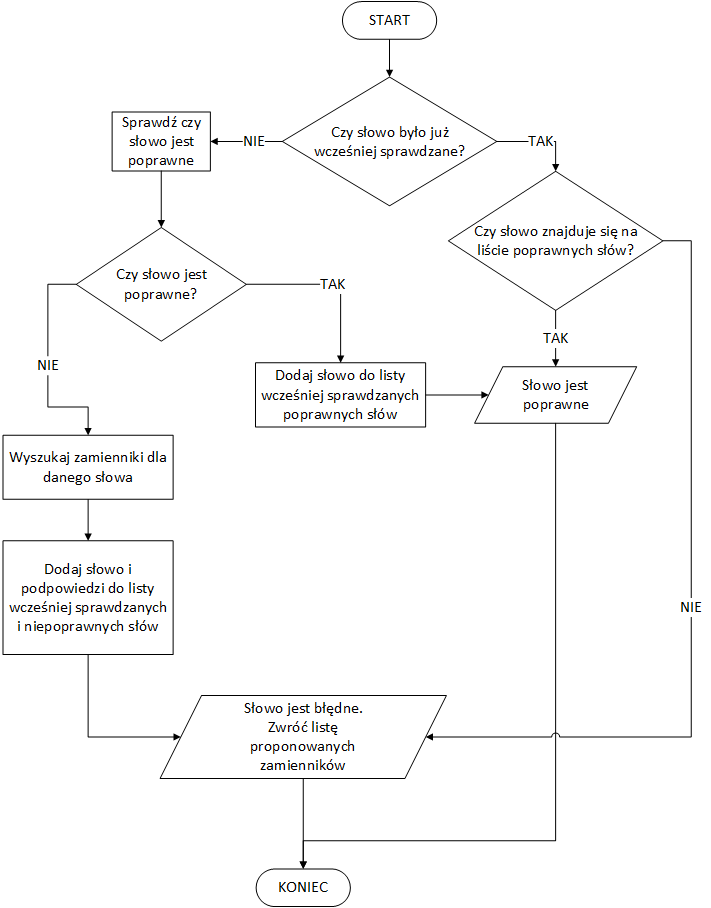
\includegraphics[width=1\linewidth]{rozdzial03/CorectorManager.png}
	\caption{Schemat korekcji tekstu z poziomu interfejsu}
	\label{fig:CorectorManager}
\end{figure}

\newpage

Główną funkcjonalnością aplikacji jest wyszukiwanie a następnie korekcja błędów. Rysunek~\ref{fig:CorectorManager} przedstawia schemat działania algorytmu odpowiedzialnego za powyższe zadanie. 

Początkowo algorytm sprawdza czy dane słowo było już wcześniej wyszukiwane. Jeśli tak to sprawdza czy jest ono na liście poprawnych słów. Jeśli tak to słowo jest poprawne i algorytm kończy pracę. Jeśli nie to sprawdza on listę błędnie wprowadzonych słów i zwraca on podpowiedzi. Jeśli podpowiedzi zostały już raz wyszukane dla danego słowa to zostają one zapisane. Ma to na celu przyspieszenie działania algorytmu ponieważ najwięcej czasu pochłania wyszukiwanie sugestii. 

Jeśli słowo jest wyszukiwane po raz pierwszy następuje sprawdzenie jego poprawności porównując je ze słowami znajdującymi się w słowniku. Jeśli jest poprawne to zostaje ono dodane do listy poprawnych sprawdzanych wcześniej słów i algorytm kończy pracę. Natomiast jeśli słowo jest błędne następuje wyszukiwanie sugestii. Po ich wyszukaniu zostają on zapisane wraz z niepoprawnym wyrazem na liście błędnych słów. Algorytm zwraca listę sugestii i kończy pracę.

Algorytm ten działa dla każdego słowa w osobnym wątku. Ma to za zadnie przyspieszenie działania aplikacji.  

